\documentclass[10pt]{beamer}
\usepackage[utf8x]{inputenc}
\usepackage{hyperref}
\usepackage{fontawesome}
\usepackage{graphicx}
\usepackage[english,ngerman]{babel}

% ------------------------------------------------------------------------------
% Use the beautiful metropolis beamer template
% ------------------------------------------------------------------------------
\usepackage[T1]{fontenc}
\usepackage{fontawesome}
\usepackage{FiraSans} 
\mode<presentation>
{
  \usetheme[progressbar=foot,numbering=fraction,background=light]{metropolis} 
  \usecolortheme{default} % or try albatross, beaver, crane, ...
  \usefonttheme{default}  % or try serif, structurebold, ...
  \setbeamertemplate{navigation symbols}{}
  \setbeamertemplate{caption}[numbered]
  %\setbeamertemplate{frame footer}{My custom footer}
} 

% ------------------------------------------------------------------------------
% beamer doesn't have texttt defined, but I usually want it anyway
% ------------------------------------------------------------------------------
\let\textttorig\texttt
\renewcommand<>{\texttt}[1]{%
  \only#2{\textttorig{#1}}%
}

% ------------------------------------------------------------------------------
% minted
% ------------------------------------------------------------------------------
\usepackage{minted}


% ------------------------------------------------------------------------------
% tcolorbox / tcblisting
% ------------------------------------------------------------------------------
\usepackage{xcolor}
\definecolor{codecolor}{HTML}{FFC300}

\usepackage{tcolorbox}
\tcbuselibrary{most,listingsutf8,minted}

\tcbset{tcbox width=auto,left=1mm,top=1mm,bottom=1mm,
right=1mm,boxsep=1mm,middle=1pt}

\newtcblisting{myr}[1]{colback=codecolor!5,colframe=codecolor!80!black,listing only, 
minted options={numbers=left, style=tcblatex,fontsize=\tiny,breaklines,autogobble,linenos,numbersep=3mm},
left=5mm,enhanced,
title=#1, fonttitle=\bfseries,
listing engine=minted,minted language=r}


% ------------------------------------------------------------------------------
% Listings
% ------------------------------------------------------------------------------
\definecolor{mygreen}{HTML}{37980D}
\definecolor{myblue}{HTML}{0D089F}
\definecolor{myred}{HTML}{98290D}

\usepackage{listings}

% the following is optional to configure custom highlighting
\lstdefinelanguage{XML}
{
  morestring=[b]",
  morecomment=[s]{<!--}{-->},
  morestring=[s]{>}{<},
  morekeywords={ref,xmlns,version,type,canonicalRef,metr,real,target}% list your attributes here
}

\lstdefinestyle{myxml}{
language=XML,
showspaces=false,
showtabs=false,
basicstyle=\ttfamily,
columns=fullflexible,
breaklines=true,
showstringspaces=false,
breakatwhitespace=true,
escapeinside={(*@}{@*)},
basicstyle=\color{mygreen}\ttfamily,%\footnotesize,
stringstyle=\color{myred},
commentstyle=\color{myblue}\upshape,
keywordstyle=\color{myblue}\bfseries,
}



%--------------------------Editor mode.

\usepackage
[citestyle=authoryear,
%style=historian, 		%Loads the Historian files
sorting=nty,	  		%Sorts bibliography by year, name, title
autocite=footnote, 		%Autocite command generates footnotes
autolang=hyphen, 			%Allows hyphenation rules for foreign languages to apply to individual entries.						%(The other language rules should all be American)
mincrossrefs=1, 		%Includes all x-ref’ed entries in the bibliography
%usetranslator=true, 	%Translator’s name may be substituted for						%author or editor, if the latter are blank
%printseries, 			%Options provided by Historian, see below
backend=biber]
{biblatex}

\DeclareFieldFormat{postnote}{#1}
\DeclareFieldFormat{multipostnote}{#1}
\DeclareAutoCiteCommand{footnote}[f]{\footcite}{\footcites}

\addbibresource{literature.bib}
\bibliography{literature}
%----------------------------------------

%--------------------------Editor mode.


%\usepackage[default]{raleway}
\usepackage{fontawesome}

\usepackage{minted}

\usepackage{hyperref}
%\usepackage{enumitem} % produces fatal error with this template

\usepackage{xcolor}
\definecolor{customcolor}{HTML}{616AC5}
\definecolor{alert}{HTML}{CD5C5C}
\definecolor{w3schools}{HTML}{4CAF50}
\definecolor{subbox}{gray}{0.60}
\definecolor{codecolor}{HTML}{FFC300}



 
%Information to be included in the title page:
\title[Pre-CLTK] %optional
{Pre-CLTK-Workshop}
\subtitle{Digitale Sprachverarbeitung für historische Disziplinen}
\institute{Zentrum für Informationsmodellierung, Graz}
\author[SL]{Sarah Lang}
\date[2019] % (optional)
{Graz, Nov. 2019}

%\logo{\includegraphics[height=1cm]{unipassau.png}\includegraphics[height=1cm]{zim.png}}



\newcommand{\punkti}{~\lbrack\dots\rbrack~}

\renewenvironment{quote}
               {\list{\faQuoteLeft\phantom{ }}{\rightmargin\leftmargin}%
                \item\relax\footnotesize\ignorespaces}
               {\unskip\unskip\phantom{xx}\faQuoteRight\endlist}

\newcommand{\bgupper}[3]{\colorbox{#1}{\color{#2}\huge\bfseries\MakeUppercase{#3}}}
\newcommand{\bg}[3]{\colorbox{#1}{\bfseries\color{#2}#3}}

\newcommand{\mycommand}[2]{{\ttfamily\detokenize{#1}}~\dotfill{}~{\footnotesize #2}\\}

\newcommand{\sep}{{\scriptsize~\faCircle{ }~}}

\newcommand{\red}[1]{\bg{alert}{white}{#1}\\}
\newcommand{\green}[1]{\bg{w3schools}{white}{#1}\\}




%----------------------------------------------------------------------------------------------------------------


\usepackage{xcolor}
\definecolor{customcolor}{HTML}{616AC5}
\definecolor{alert}{HTML}{CD5C5C}
\definecolor{w3schools}{HTML}{4CAF50}
\definecolor{subbox}{gray}{0.60}
\definecolor{codecolor}{HTML}{FFC300}


%--------------------------------------------------------------------------------
\usepackage{tcolorbox}

\tcbuselibrary{most,listingsutf8,minted}

\tcbset{tcbox width=auto,left=1mm,top=1mm,bottom=1mm,
right=1mm,boxsep=1mm,middle=1pt}

\newenvironment{mycolorbox}[2]{%
\begin{tcolorbox}[grow to left by=-1em,grow to right by=-1em,capture=minipage,fonttitle=\large\bfseries, enhanced jigsaw,boxsep=1mm,colback=#1!30!white,on line,tcbox width=auto, toptitle=0mm,colframe=#1,opacityback=0.7,nobeforeafter,title=#2]\scriptsize%
}{\end{tcolorbox}\\[0.2em]}

\newenvironment{subbox}[2]{%
\begin{tcolorbox}[capture=minipage,fonttitle=\normalsize\bfseries, enhanced jigsaw,boxsep=1mm,colback=#1!30!white,on line,tcbox width=auto,left=0.3em,top=1mm, toptitle=0mm,colframe=#1,opacityback=0.7,nobeforeafter,title=#2]\scriptsize %
}{\normalsize\end{tcolorbox}\vspace{0.1em}}

\newenvironment{multibox}[1]{%
\begin{tcbraster}[raster columns=#1,raster equal height,nobeforeafter,raster column skip=1em,raster left skip=1em,raster right skip=1em]}{\end{tcbraster}}


\newenvironment{mycodebox}[2]{%
\begin{tcolorbox}[grow to left by=-1em,grow to right by=-1em,capture=minipage,fonttitle=\large\bfseries, enhanced jigsaw,boxsep=1mm,colback=#1!30!white,on line,tcbox width=auto, toptitle=0mm,colframe=#1,opacityback=0.7,nobeforeafter,title=#2]%
}{\end{tcolorbox}\\[0.2em]}

\newtcolorbox{mybox}[2][]{colback=codecolor!10!white,coltitle=red!70!black,
title={#2},fonttitle=\bfseries,#1}


%-------------------------------

\newtcblisting{mypy}[1]{colback=codecolor!5,colframe=codecolor!80!black,listing only, 
minted options={numbers=left, style=tcblatex,fontsize=\scriptsize,breaklines,autogobble,linenos,numbersep=3mm},
left=5mm,enhanced,
title=#1, fonttitle=\bfseries,
listing engine=minted,minted language=python}

\newtcblisting{myxml}[1]{colback=codecolor!5,colframe=codecolor!80!black,listing only, 
minted options={numbers=left, style=tcblatex,fontsize=\tiny,breaklines,autogobble,linenos,numbersep=3mm},
left=5mm,enhanced,
title=#1, fonttitle=\bfseries,
listing engine=minted,minted language=xml}

\newtcblisting{mybiggerxml}[1]{colback=codecolor!5,colframe=codecolor!80!black,listing only, 
minted options={numbers=left, style=tcblatex,fontsize=\footnotesize,breaklines,autogobble,linenos,numbersep=3mm},
left=5mm,enhanced,
title=#1, fonttitle=\bfseries,
listing engine=minted,minted language=xml}

\newtcblisting{myhtml}[1]{colback=codecolor!5,colframe=codecolor!80!black,listing only, 
minted options={numbers=left, style=tcblatex,fontsize=\tiny,breaklines,autogobble,linenos,numbersep=3mm},
left=5mm,enhanced,
title=#1, fonttitle=\bfseries,
listing engine=minted,minted language=html}

\newtcblisting{mycss}[1]{colback=codecolor!5,colframe=codecolor!80!black,listing only, 
minted options={numbers=left, style=tcblatex,fontsize=\tiny,breaklines,autogobble,linenos,numbersep=3mm},
left=5mm,enhanced,
title=#1, fonttitle=\bfseries,
listing engine=minted,minted language=css}


\newtcblisting{myjs}[1]{colback=codecolor!5,colframe=codecolor!80!black,listing only, 
minted options={numbers=left, style=tcblatex,fontsize=\tiny,breaklines,autogobble,linenos,numbersep=3mm},
left=5mm,enhanced,
title=#1, fonttitle=\bfseries,
listing engine=minted,minted language=js}

% ------------------------------------------------------------------------------
% The Document
% ------------------------------------------------------------------------------
\title{Pre-CLTK-Workshop}
\author{Sarah Lang}
\date{Nov.2019}

\begin{document}

\maketitle

\begin{frame}{TOC}
\tableofcontents
\end{frame}

\section{Intro}
\subsection{Python-Installation}

\begin{frame}[fragile,allowframebreaks]{Python Installation}
\begin{enumerate}
    \item Wir wollen die Anaconda Distribution installieren.
    \item Wer hat das schon? Wer braucht das noch?
    \item Welche Probleme gab es?
    \item Danach müssen noch NLTK und CLTK installiert werden (dauert einen Moment!)
\end{enumerate}

\framebreak
\red{Linux-Bug} (ggf. Fehlermeldung `conda not found')

\href{https://support.anaconda.com/hc/en-us/articles/360023863234-Conda-command-not-found-error}{Support:Conda not found error} \sep \href{https://support.anaconda.com/hc/en-us/articles/360024042553-Anaconda-Navigator-Issues-Launching-or-Initializing}{Support Navigator Issues}
$\to$ dann:

\mycommand{export PATH=~/anaconda3/bin:$PATH}{Path fehlt}
\mycommand{conda --version}{check if working}
\mycommand{conda init}{initialize}
\mycommand{anaconda-navigator}{launch navigator}

When started: Click Jupyter Notebook. Choose directory. New $\to$ Python 3.
    
\end{frame}

\subsection{Erste Schritte in Jupyter / NTLK-Installation}
\begin{frame}[fragile, allowframebreaks]{Erste Schritte in Jupyter / NTLK-Installation}
\begin{minted}[fontsize=\footnotesize]{py}
# press CTRL+ENTER to evaluate in Jupyter
# mit '#' markiert man Kommentare, 
# also Infos für sich selbst, die der Computer aber ignorieren soll
1 * 4 + 5 / 8
# wie funktionieren die Klammern??

# Grundlegende Funktionalitäten sind bereits in der
# Standard-Bibliothek enthalten. Für Spezielleres 
# müssen wir sog. 'Pakete' hineinladen. 
# Das geht z.B. so:
import nltk 
nltk.download() # Der Schritt ist nur 1x nötig, 
# wenn das halt noch nicht installiert ist oder 
# out-of-date oder man nicht alles gedownloaded 
# hat beim letzten Mal und jetzt noch andere Sachen
# dazunehmen will (Paket ist relativ groß, 
# daher könnte es von Interesse sein, nur selektiv manche Sachen zu nehmen)

# nicht vergessen im Prompt/Dialog zu klicken, 
# was man will (Progressbar startet), sonst passiert nix

from nltk.book import *
text1 # Moby Dick
\end{minted}
    
\end{frame}

\section{Theorie}
\begin{frame}{Begrifflichkeiten}
    
Quantitative methods in literary studies began in the sub-field of Stylometry: 
L.A. Sherman \emph{Analytics of Literature} (1893).  Now, there are many sub-fields and different names for quantitative methods for texts and language processing\footcite[\scriptsize A fascinating introductory read on the `statistical language model', underlying computerized language processing, is][\scriptsize Don't be put off by the emphasis on mathematics, it's really a series of easy-to-understand blog posts about langauge processing.]{beautyOfMathematics} in/for the Humanities:

\red{Quantitative Text Analysis (QTA)} \green{Computational Literary Studies (CLS)}

\red{Computational Linguistics} 

\green{Text Mining}
\red{Franco Moretti's \emph{Distant Reading}}
\red{Matthew Jocker's \emph{Macroanalysis}}

\end{frame}

\begin{frame}{Funktionen}
\begin{enumerate}
    \item \red{exploratory} Exploring a corpus for potentially interesting patterns. Be pointed to interesting phenomena; find new research questions; explore the `potentials' of the text/corpus.
    \item \red{descriptive} Describing phenomena quantitatively which we already `feel' are there but we want to grasp them more `objectively'. Confirm `qualitative hypotheses quantitatively.
    \item $\to$ both are not `results'! They still require interpretation to be valid for Humanities purposes.
\end{enumerate}
\end{frame}






\section{Intro to NLP concepts}

\begin{frame}[allowframebreaks]{Basic concepts I}
\red{Bag-of-words (BOW)}
\green{\emph{type} vs. \emph{token}}
\emph{To be or not to be.} = 6 \emph{tokens}, 4 \emph{types}.
$\to$ aus den \emph{types} wird der \emph{bag of words} aufgebaut, darin werden dann alle Vorkommnisse (\emph{tokens}) gezählt.

\red{\emph{type}} beschreibendes Kriterium

\red{\emph{token}} Analyseeinheit

\green{\emph{case-folding}} alles in \emph{lowercase} analysieren: hat vor und Nachteile (z.B. Eigennamen), am Satzanfang evtl. sinnvoll, außer für Stilometrie. Stattdessen evtl.
\green{\emph{truecaseing}}

Je nach Entscheidung bzgl. \emph{case-folding/truecasing} ist ein Wort in Großschreibung ein anderer \emph{type} als in Kleinschreibung!
\end{frame}

\begin{frame}[allowframebreaks]{Bag-of-words}

\underline{Was geht dabei alles verloren?}
\begin{itemize}
    \item Wortstellung
    \item Zusammenhang
    \item Phrasen
    \item Reihenfolge
    \item Ironie, Sarkasmus, Negation
\end{itemize}
\end{frame}

\begin{frame}[allowframebreaks]{Basic concepts II}

\green{Zipf'sche Verteilung (\emph{Zipf's Law})} starker (proportionaler) Abfall der Häufigkeit (und absoluten Streuung) mit zunehmendem Rang 
\begin{quote}
Zipf's law states that given a large sample of words used, the frequency of any word is inversely proportional to its rank in the frequency table. (Wikipedia) \end{quote}

\red{Stopwords} überproportional häufige Wörter (und, \emph{the}, etc.). In Listen gesammelt, meist aus der Analyse entfernt, da sie die interessanten Partien `verdecken'.
\emph{To be or not to be} = alles Stopwords.

\red{Wortfrequenzanalysen} siehe `Statistische Grundlagen'
\end{frame}

\begin{frame}[allowframebreaks]{Unigramme Bigramme n-Gramme}

\red{Unigramme vs. n-Gramme}
\textbf{Unigram}: Jeglicher Kontext geht verloren. \\
\textbf{n-Gramme}: 
\green{\emph{sparse data}-Problem} d.h. wir haben fast nie genug Daten dafür, außer bei \emph{sehr} großen Korpora. Die Häufigkeiten werden dabei schnell so `selten', dass nichts statistisch Relevantes mehr dabei ist. Mehr als 3-5-Gramme sind daher nicht üblich. (zumal für historische Sprachen ohnehin viel zu kleine Korpora erhalten sind!)

\end{frame}


\begin{frame}[allowframebreaks]{Basic Concepts III}
\green{KWIC (=Keyword in Context)} 
\green{Kollokation}
\green{Konkordanz}

\begin{quote}\tiny
    Unter Konkordanz (zurückgehend auf lat. \emph{concordare} „übereinstimmen“), versteht man in den Textwissenschaften traditionellerweise eine alphabetisch geordnete Liste der wichtigsten Wörter und Phrasen, die in einem schriftlichen Werk verwendet werden. Der Begriff stammt aus der Bibelwissenschaft. \punkti

    Konkordanzen sind heute in der Regel elektronisch erstellte Trefferlisten, die sich aus der Suche meist nach einem Wort oder einer Phrase, eigentlich aber aus der Suche nach jeder beliebig definierbaren Zeichenkette ergeben. In einer Konkordanz ist meistens auch die nächste sprachliche Umgebung des gesuchten Ausdrucks, der sogenannte \emph{Kontext} angeführt, also beispielsweise der gesamte Satz, in dem ein gesuchtes Wort auftritt.
    
    Als Synonyme für Konkordanz gelten fallweise die Ausdrücke \emph{Register} und \emph{Index} oder \emph{Index verborum} (‚Verzeichnis der Wörter‘). 
    
    In der Korpus- und in der Computerlinguistik haben sich zudem, auch im Deutschen, der Ausdruck \emph{Key Word in Context} sowie dessen Abkürzung \emph{KWIC} als Benennungen für den in einer Konkordanz angezeigten Suchbegriff eingebürgert.  (\href{https://de.wikipedia.org/wiki/Konkordanz_(Textwissenschaft)}{Wikipedia})
\end{quote}

\end{frame}

\begin{frame}[allowframebreaks]{Sentiment Analysis}
\red{\emph{Sentiment Analysis}}
Eine weitere bekannt gewordene `Wörterbuch-Methode'. Man macht quasi ganz normal die Auszählung und verbindet dann die Tabelle per \emph{join} mit einem \emph{sentiment dictionary}, das Wörter in Kategorien bewertet. Allerdings passieren natürlich Missverständnisse: Bsp: Jane Austens häufigstes Nicht-Stopwort ist `Miss', aber in \emph{lowercase} (da \emph{case-folding}) wird es natürlich fehltinterpretiert als `vermissen' und damit als negatives Gefühl gewertet!
\end{frame}

\begin{frame}[standout]
Hintergrundinfos zu \alert{statistischen Grundlagen} und \alert{Korpusaufbau} siehe Cheatsheet! \\
\footnotesize Bitte ggf. selbst aneignen / einlesen.
\end{frame}




\begin{frame}[allowframebreaks]{Konzepte bzw. Theorien der QTA}
\begin{quote}
    Reading `more' seems hardly to be the solution. Especially because we've just started rediscovering what Margaret Cohen calls the `great unread'. \lbrack{} Apart from ``its canonical fraction, which is not even 1 per cent of published literature''\rbrack{} there are \lbrack{}thousands of books\rbrack{} -- no one really knows, no one has read them, no one ever will.\footcite[45]{distantreading} 
\end{quote}

\red{Franco Morettis \emph{Distant Reading}} 
Vorstellung serielles Lesen vs. menschliches \emph{Close Reading}. 
Behauptet, Literaturwissenschaft wäre nicht mehr vollständig ohne quantitative Aspekte. Das serielle Lesen aber auch irgendwie `als Alternative' anstatt \emph{close reading}.

\begin{quote}
    \punkti you \emph{reduce} a text to a few elements, and \emph{abstract} them from the narrative flow, and construct a new, \emph{artificial} object. \punkti And with a little luck, these maps will \punkti possess `emerging' qualities, which were not visible at the lower level. \punkti Not that the map itself is an explanation, of course. It offers a model \punkti\footcite[53]{graphsmoretti} 
\end{quote}


\bigskip

\green{Matthew Jockers's \emph{Macroanalysis}}
Vorstellung einer Zoom-Bewegung: Die quantitative Analyse bietet Anstöße für das \emph{Close Reading}, etc.
Er fordert die Unterscheidung zwischen \emph{reading} und \emph{analysis} -- der Überblick `aus der Ferne' ist für ihn nicht `Lesen', wie etwa Morettis Benennung suggerieren würde.
\begin{enumerate}
    \item Kontextualisierung durch das \emph{zooming out}
    \item andererseits aber auch extremes \emph{close reading}: So viel Details wie dem Computer können einem Menschen fast gar nicht auffallen, weil wir Details ja gar nicht so richtig wahrnehmen.
    \item besser informiertes Verstehen der Primärtexte: die \emph{macroscale} gibt weniger `anekdotische' Beweise als das sehr genaue Lesen nur eines einzigen Texts.
    \item `harvesting findings, not facts'
\end{enumerate}

`Mixed Methods'-Ansatz, Wechselspiel

\begin{quote}
    This is not close reading; this is macroanalysis, and the strength of the approach is that it allows for both zooming in and zooming out.\footcite[23]{macroanalysis}
\end{quote}

\red{Pipers \emph{cultural analytics}}

\end{frame}


\section{NLP-Pipeline}
\begin{frame}[allowframebreaks]{NLP-Pipeline}
\red{(\emph{Pre-Processing})}
$\to$ fällt in unserem Fall normalerweise unter das sog. (\emph{Pre-Processing})

\red{Tokenizer}
\textbf{Einfachste Tokenizer:} Nur der Whitespace/Leerzeichen ist Trenner. Erweiterbar durch Hinzufügen von Punktuation oder sprachinternen Spezifika.

\textbf{Sprachgebunden}, z.B. frz. \emph{l'enfant}, lat. \emph{dixitque}, en. \emph{don't} auflösen, \dots 

Wie wird mit \textbf{\emph{compounds}} (zusammengesetzen Wörtern) umgegangen?
Fremdsprachliche \textbf{Lehnwörter}, die zusätzlich noch stehende Wendungen sind (z.B. \emph{en masse})?

Geht meist ohne Wörterbuch -- für die meisten anderen NLP-Methoden müssen Wörterbücher und Grammatiken vorliegen (! ist für einen historischen Sprachstatus absolut nicht selbstverständlich) $\to$ Computer kann nicht denken und ist z.B. mit der uneinheitlichen Orthographie von frühneuzeitlichem Deutsch völlig überfordert: Methoden davon teilweise in die völlige Impraktikabilität reduziert! 

$\to$ aber geht natürlich super für moderne lebendige Sprachen, v.a. Englisch.

\begin{quote}
    \textbf{But what is a word?} We tend to think of a word as a unit of meaning that often has an analog in the real world. \punkti A computer doesn't know what a word is and certainly has no sense of what words might refer to.
    \punkti 
    Words are usually bounded by spaces and punctuation, and a computer can be told to split a long string (text) into shorter strings (words) by looking for the demarcation characters \punkti -- a process called tokenization.\footcite[283]{textvisual}
\end{quote}
\end{frame}


\begin{frame}[allowframebreaks]{Im Detail dazu im Praxisteil}

\red{Lemmatization} Mithilfe von \textbf{Wörterbuch/Vokabular, Grammatik und morphologischer Analyse} der Wörter die Grundform (das \emph{Lemma}, wie man es im Wörterbuch hat) zu finden, damit alle Wortformen korrekt als Formen desselben \emph{type} gezählt werden können.

\red{Stemming} Wortende bis zur Wurzel abschneiden, nicht unbedingt auf linguistisch korrekte Art und Weise.

\red{Parsing}

\red{POS tagging}

\end{frame}

\begin{frame}{Buch-Tipps zum Einstieg}

\href{https://www.springer.com/de/book/9783476026224}{
\includegraphics[width=0.45\textwidth]{dh-einf.png}}
\hspace{2em}
\href{https://www.nltk.org/book/}{
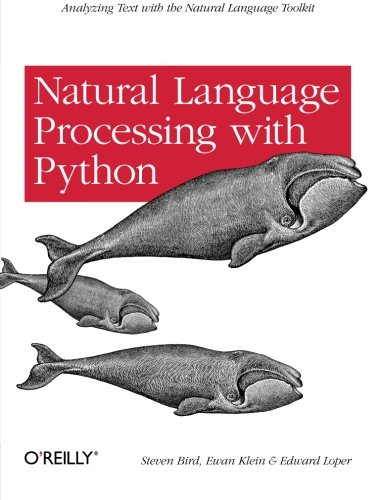
\includegraphics[width=0.45\textwidth]{nltk-buch-python.jpg}
}
\end{frame}


\section{Tools und Visualisierung}


\begin{frame}[allowframebreaks]{Informationsvisualisierung (\emph{`DataViz' / `InfoViz'})}
Siehe Kapitel 23 `Informationsvisualisierung' (DH-Einführungsbuch)\footcite[vgl.][]{DHIntroRehbeinInfoviz}


Grafische Elemente als Kommunikationsmittel \sep
visuelle statistische Darstellungen als Repräsentationen von Sprache \sep
Entlastung des Geistes bei großes Datenmengen: \emph{snapshot} statt Gesamtwerk. \sep `method for seeing the unseen' \sep durch die Visualisierung werden abstrakte Daten räumlich angeordnet \sep oft interaktive Schnittstellen, um den Denkprozess zu begleiten 

\framebreak
\green{Funktionen}
\begin{enumerate}
\item \textbf{anschauliche Präsentation} von Daten/Ergebnissen, am Ende des Forschungsprozesses
\item \textbf{konfirmative Analyse:} Sichweisen (\emph{views}) auf Daten erzeugen, die erlauben, Hypothesen zu verifizieren oder falsifizieren. Teil des Forschungsprozesses.
\item \textbf{explorative Analyse:} nicht hypothesengetrieben, Strukturen oder Trends erkennen. $\to$ interaktive Werkzeuge, zu Beginn des Forschungsprozesses
\item \textbf{Visualisierung} (z.B. Storytelling)
\end{enumerate}

\red{makros vs. mikro} Einerseits Aufzeigen übergeordneter Strukturen (`distant reading'), aber auch Detaileinblick in die Daten.

\green{Vorgehen}
\emph{raw data} $\to$ (Vorverarbeitung) $\to$ \emph{data tables} $\to$ \emph{visual structures} $\to$ \emph{views}.

$\to$ Tufte 1983: \emph{A silly theory means a silly graphics.}
% bis S. 334: weiter mit Datentypen, visuelle Strukturen
\end{frame}

\begin{frame}[allowframebreaks]{Nie vergessen}

\begin{quote}\normalsize
        \emph{A fool with a tool is still a fool!} (\href{https://en.wikiquote.org/wiki/Talk:Grady_Booch}{Grady Booch})
    \end{quote}

\end{frame}



\begin{frame}[allowframebreaks]{DataViz III}
\green{Frage nach der Aussagekraft der Daten}
\begin{quote}\small
Nur aus der bloßen Existenz von Daten kann nicht auf deren Bedeutsamkeit geschlossen werden, und nicht alles, was (in einem bestimmten Kontext) bedeutsam ist, hinterlässt messbare Datenspuren.

Ein weiterer Schritt ist durch den Forscher selbst zu vollziehen: Visualisierungen sind häufig gut geeignet, um Strukturen und Muster zu zeigen. Sie liefern allein für sich aber keine Erklärungen. Mit anderen Worten: Korrelationen oder Koinzidenzen, wie sie sich vielleicht in den Daten erkennen lassen, bedeuten noch keine Kausalität, eine Wiederkehr noch keine Gesetzmäßigkeit. Erklärungen lassen sich erst durch Interpretation der Visualisierungen, oft unter Bezugnahme von anderen Daten, Quellen oder auch Methoden, durch den Forscher folgern. \emph{(Rehbein 2017, 341--341)}
\end{quote}
\end{frame}


\begin{frame}{Rolling Window}
\href{http://www.thomaswilhelm.eu/shakespeare/output/hamlet.html}{To See Or Not to See: Shakespeare-Visualisierung} \sep Annotationsbasiert

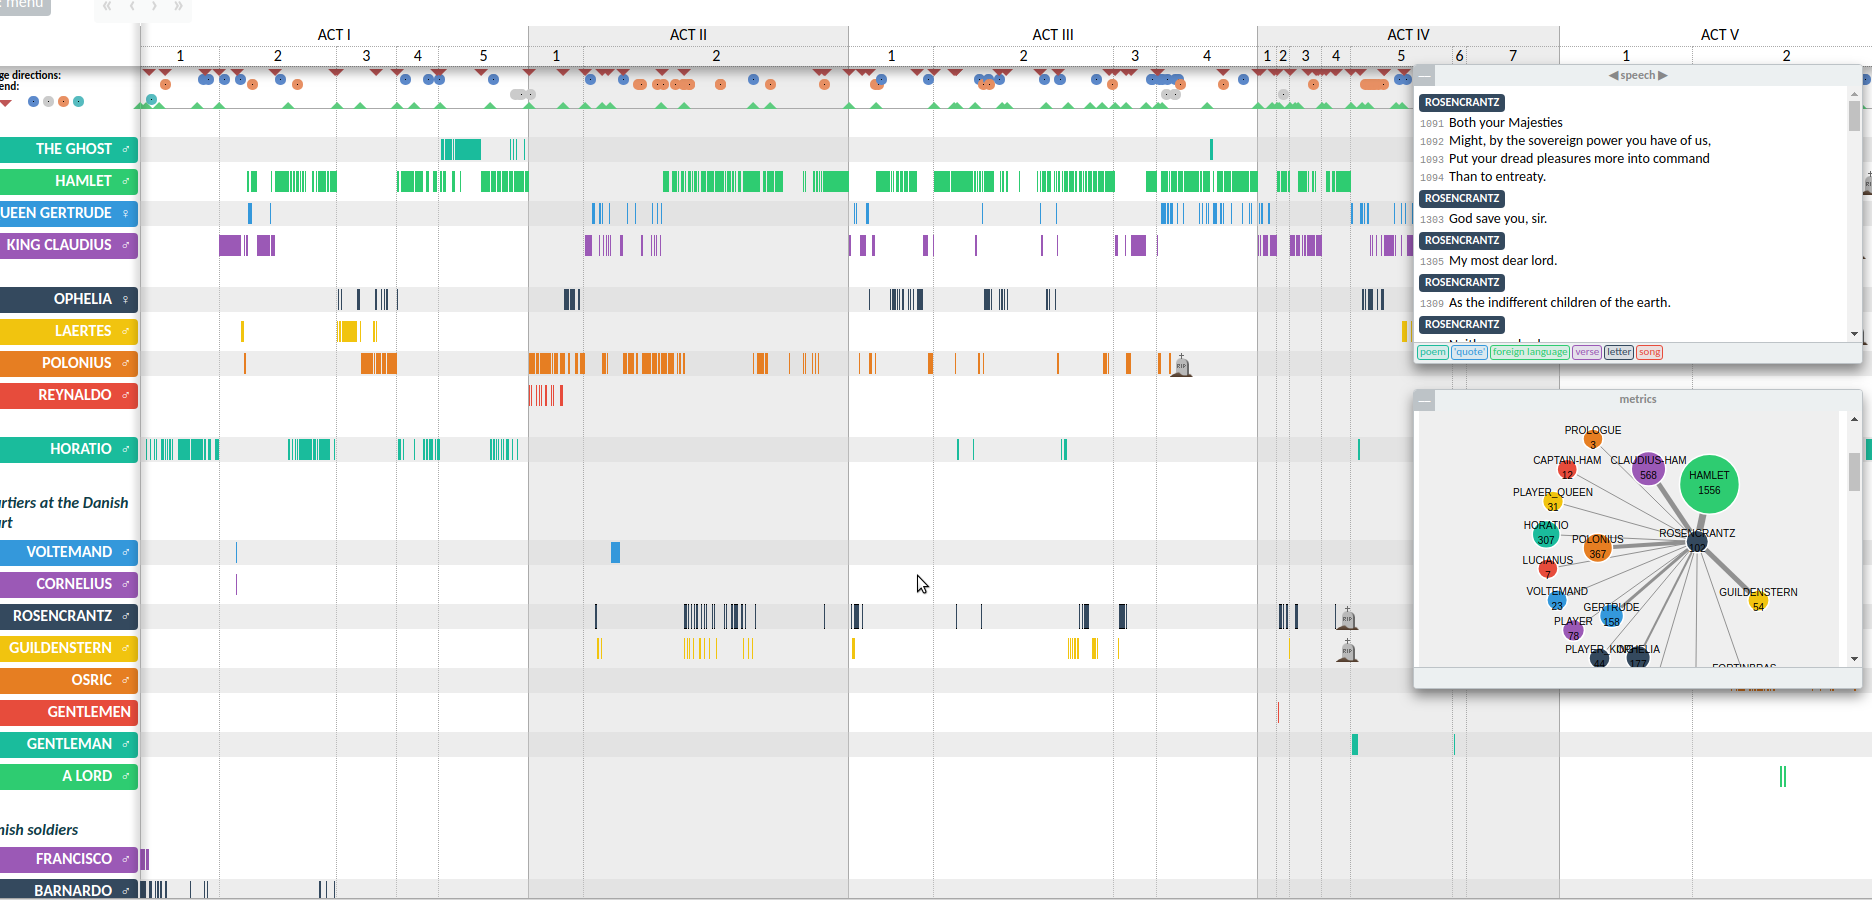
\includegraphics[width=\textwidth]{toSeeOrNotToSee.png}
\end{frame}


\begin{frame}{\href{https://www.jasondavies.com/wordtree/}{WordTree}}

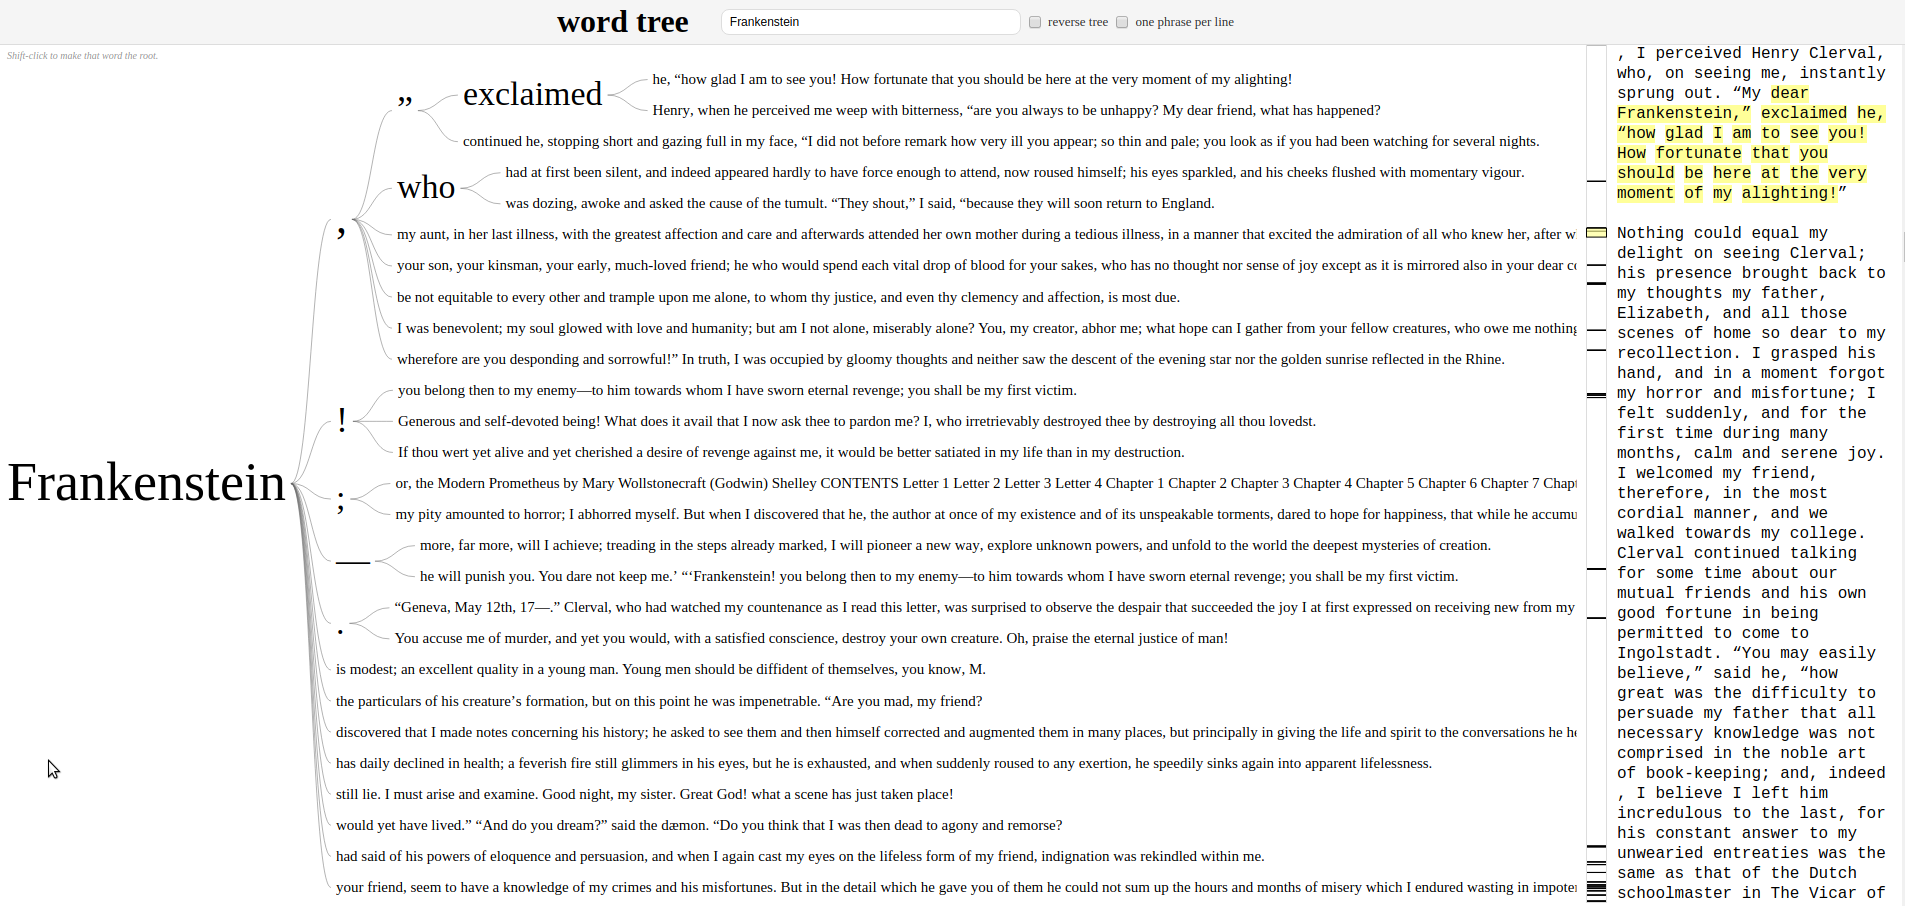
\includegraphics[width=\textwidth]{wordTree.png}
\end{frame}

\begin{frame}{\href{https://voyant-tools.org/}{Voyant Tools}}
\href{https://blogs.reed.edu/ed-tech/2017/03/text-analysis-using-voyant-tools/}{Blogpost zu Voyant} \sep features many standard functions for single and multiple documents \sep XML input possible as well

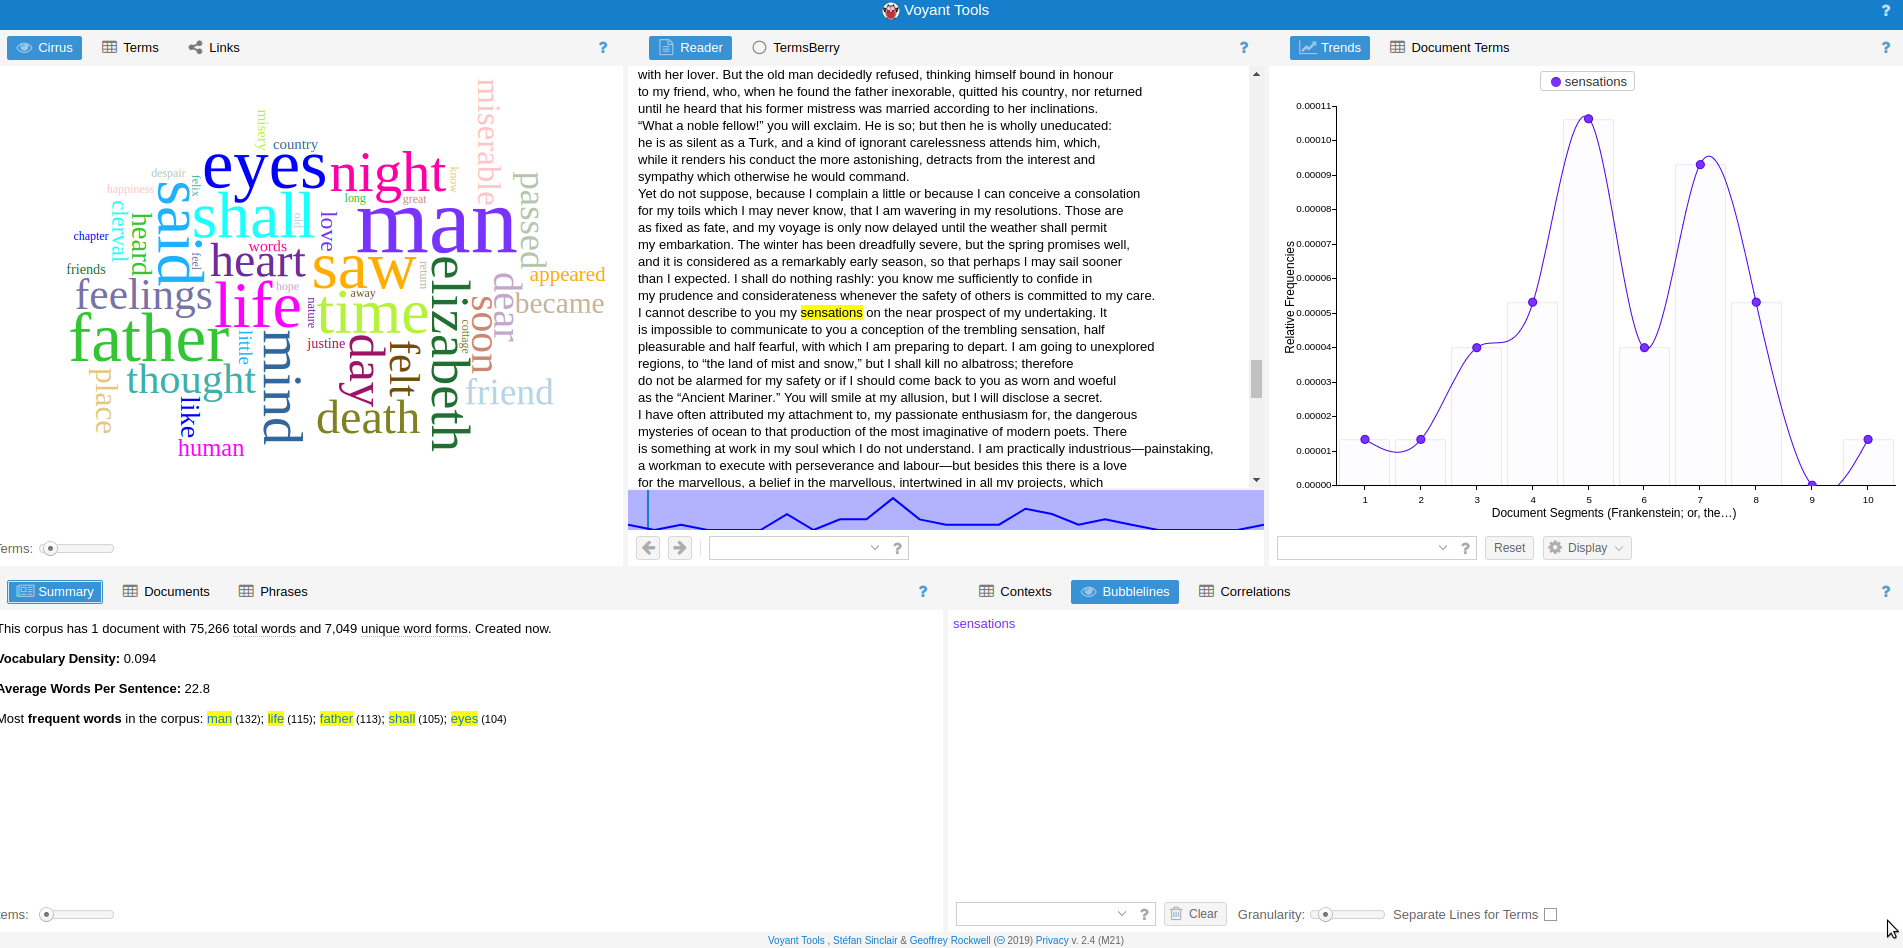
\includegraphics[width=\textwidth]{voyant.png}
\end{frame}



\begin{frame}{\href{https://books.google.com/ngrams}{Google Books N-Gram Viewer}}
\href{https://firstmonday.org/ojs/index.php/fm/article/view/5567/5535}{Shai Opir: Bsp. zu `Truth'}

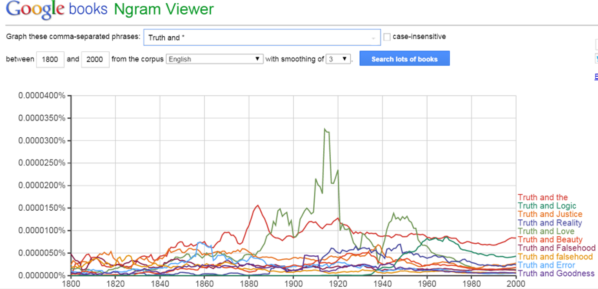
\includegraphics[width=\textwidth]{googlengramstruth.png}
\end{frame}

\begin{frame}[allowframebreaks]{NLP-Tools}
\bg{w3schools}{white}{Stanford CoreNLP} \\
\href{https://stanfordnlp.github.io/CoreNLP/tutorials.html}{Stanford CoreNLP} \sep 
\href{https://corenlp.run/}{Online-Tool für CoreNLP} \sep 
\href{https://interviewbubble.com/getting-started-with-stanford-corenlp/}{Einsteiger-Tutorial zu CoreNLPs Funktionen}

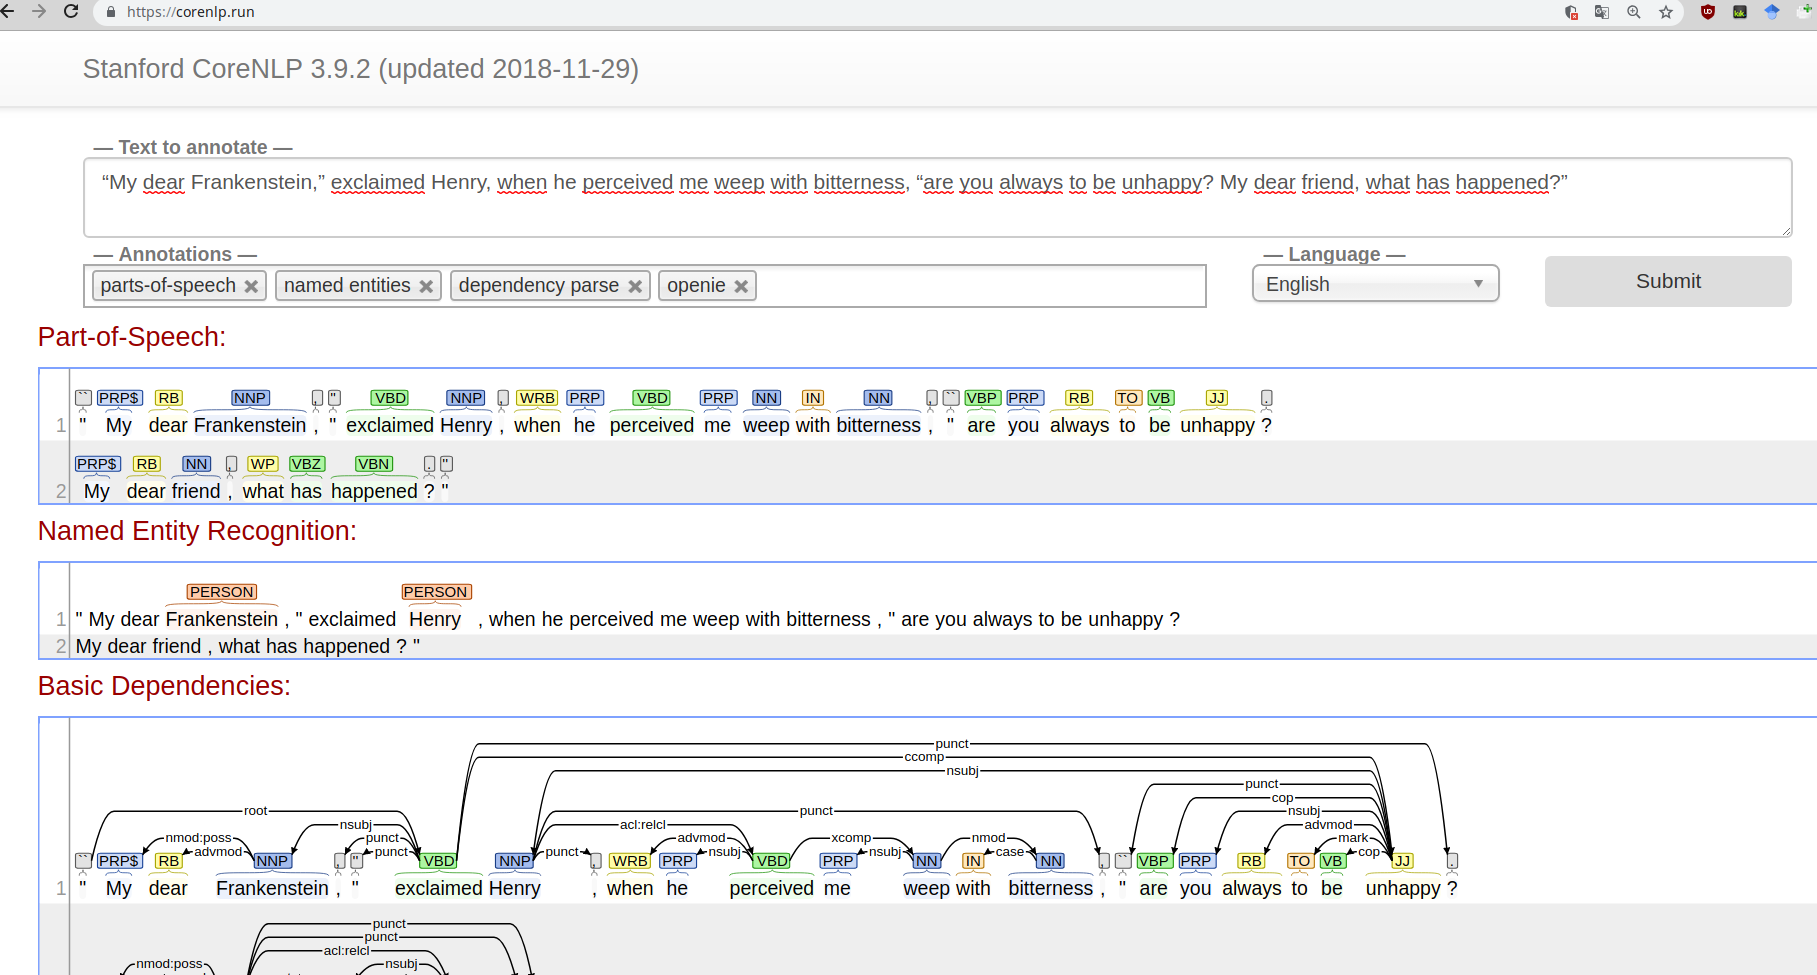
\includegraphics[width=\textwidth]{frankenstein-corenlp.png}


\href{http://www.wordandphrase.info/}{Word and Phrase}: Konkordanzen, Frequenzlisten, Texte analysieren (ein ganzer Roman scheint ihm zu viel zu sein)

\end{frame}



\begin{frame}[allowframebreaks]{\href{http://wordwanderer.org/}{WordWanderer}}
Konkordanz, Beziehungen zu anderen Wörtern, etc. Vom einen Begriff zum nächsten hangeln, \dots

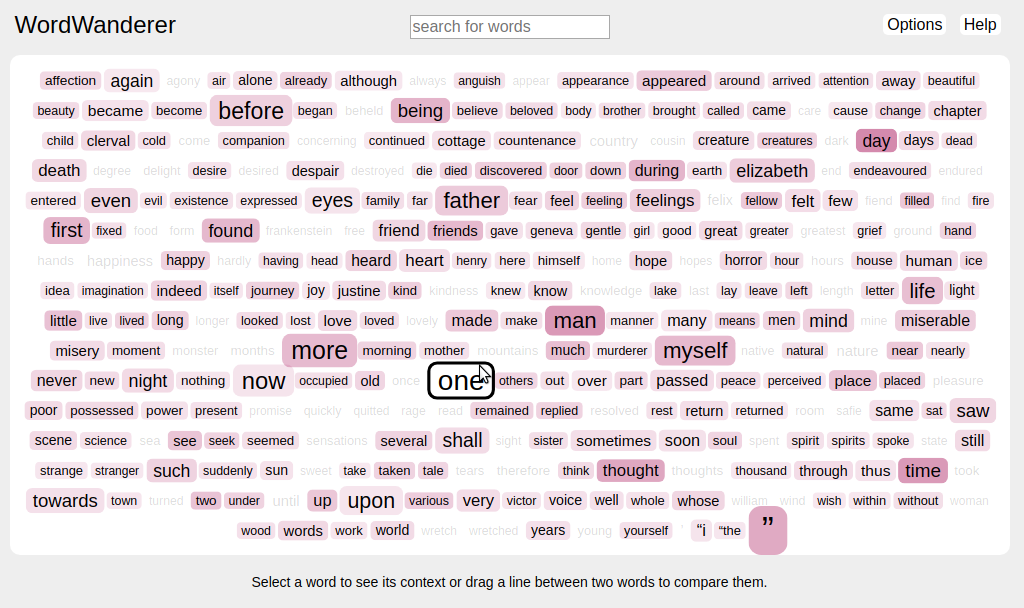
\includegraphics[width=\textwidth]{wordwanderer1.png}

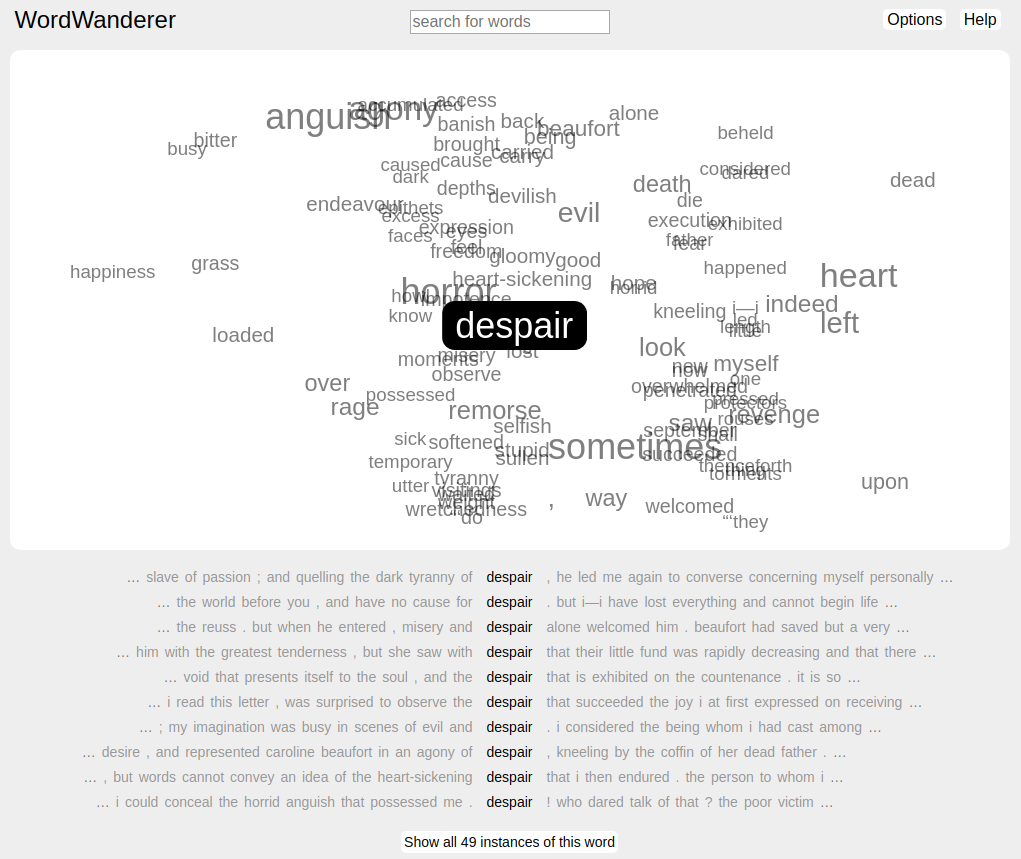
\includegraphics[width=\textwidth]{wordwanderer2.png}

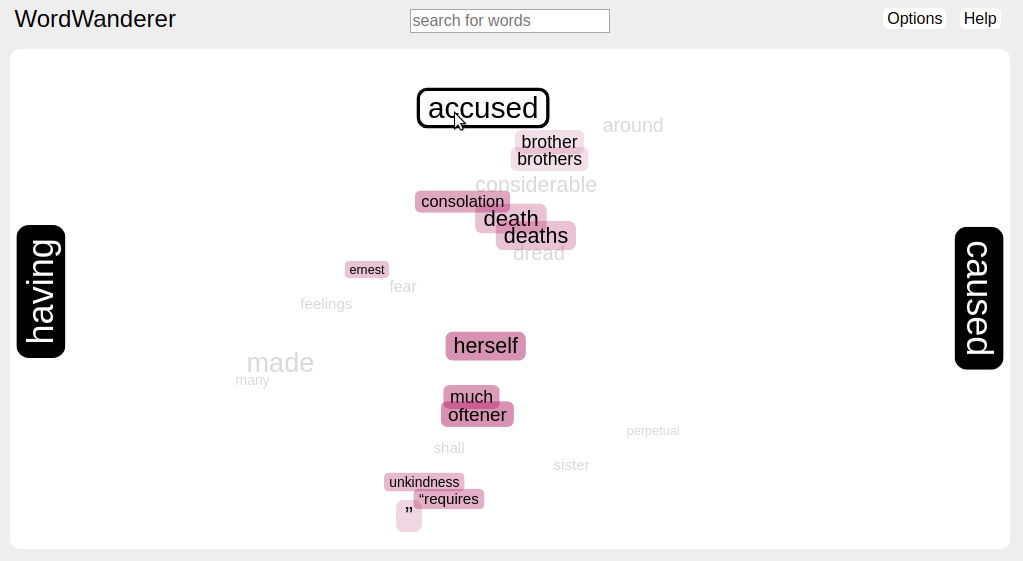
\includegraphics[width=\textwidth]{wordwanderer3.png}
\end{frame}




\section{Grundbegriffe der Programmierung}

\begin{frame}[allowframebreaks]{Communicating with computers}
\footnotesize
\green{Algorithm} Recipe providing a formalized way to automate carrying out a task.

can be in `pseudo-code' (``Whenever you find a verb, do this. When you find a noun, do that.'' etc.)

\green{Algorithmic thinking} The art of communicating effectively with a computer

\green{Debugging} is the art of error correction There are different types of errors, most importantly:

\red{Syntax errors} mean that you didn't respect the conventions of your programming language. \textasciitilde Typos

\red{Logic errors} \textasciitilde design flaw. Usually these are `bigger' errors in the program flow compared to the more localized syntax errors (typos, missing semicolon or closing brackets, etc.).

\red{Semantic errors} mean that the code runs alright, but it doesn't do what you intended it to do.

\red{Runtime error} A program crashes due to unexpected input but the compiler can't know someone will input something which will cause the crash (such as an unexpected and thus uncaught division-by-zero error which you should actually prevent). There are many recurring types of errors which consequently have received their own names, such as index-out-of-range error or off-by-one error, to name to most well-known examples.


\red{Error handling} Errors should be handeled in your program flow, this means they should be anticipated, `caught' or `thrown'. An error message will specify what kind of problem happened which makes debugging easier. An expected and thus properly handeled error prevents the program from crashing whenever something problematic happens (which shouldn't happen!). If you have an advanced error handling in place, your program will know how to react when different types of errors happen. However, this is maybe overkill for tiny script-like programs where a crash is not an issue. 

\green{Input and Output} Input and output (sometimes referred to as I/0) are base concepts of how computing works: You give input to a function or computer program and expect it to return a certain output. In between, some processing happens.

\green{Variable} A variable is a container for storing information. A variable is a container for storing information, kind of like in maths where a variable is a placeholder for a yet unkown value. It is named (such as 'x' in maths). Calling the name usually causes it to give you its `contents'.

\green{Function} A function is a generalized bit of code, made for general-purpose reuse. So essentially, you abstract what is being done. Instead of ``process my document test.txt'' you would write something like \texttt{process(text)} and would be able to pass a document of any name to this \texttt{process()} function like \texttt{process("test.txt")} or \texttt{process("unicorn.txt")}. This has the awesome advantage that it doesn't matter whether your document is called `test' or `unicorn' or, in fact, any other crazy name you can come up with. A function usually has a `signature' that means a list of what parameters you pass to it (in the definition of a function, you say which type of data will be inputted) and what it will return.

\green{Parameter} is a variable in the declaration of a function. Together with variables (and parameters \emph{are} a type of variable), parameters contribute to the abstraction of functions. This is a good thing. 

\green{Argument} is almost the same as a parameter, but the difference is that it means the actual value which gets passed to the function. So when using a function, you can pass the number 3 to it. In the definition/declaration, you say that an integer variable will be passed to it (=the parameter is an integer type value). 

\green{Return value} What a function will return as a result. This has a `return type', specifying which data type will be returned.  This can sometimes be good to know so that we don't get confused in further processing steps. 

However, the point about the whole function-abstraction-thing is that we really shouldn't need to know exactly how the processing is done in a function. We only need to know what we put int (input) and what we expect to get out of it (output). This makes it easier to build really complex programs where you don't want to have to worry about how excatly things were implemented in the detailled single processing steps.


\green{Library} A library (or package) is essentially nothing else than a bunch of functions, only that when you load them into your program, you can profit from (usually) really well-done and maintained functions somebody else made. 

When you use code from a library, it means that this code is not part of the standard repertoire (`vocabulary') of your language: It is a set of functions made using this standard repertoire just as your own functions are. When you invoke or `load' them, it's essentially as though the computer would just copy their text into your document behind the scenes (and this is exactly what happens behind the scenes). 

Functions coming from libraries can have the name of their library prefixed as a `namespace'. This can sometimes be a little confusing, especially for beginners because it obscures where which names belong to in longer expressions and requires you to know/remember from which libraries your used functions come.

\textbf{Redundancy is always an unnecessary source of error.} Avoid redundancy at all costs. Except for in data archiving. Here, redundancy is security.

\red{Divide et impera}
In the beginning, we learned that an algorithm (and thus, also it's concrete \emph{implementation}, a program) is essentially a cooking recipe which allows us to automate things which are simple enough so they lend themselves to being automated. Sometimes, even things which look complicated at first can be reduced to simpler substeps. This is called the \textbf{`divide et impera' principle} in computer programming. 

However, cooking recipes always expect the same input (the ingredients, so to speak). If the input differs from what's specified (even just a tiny little bit!), the computer really doesn't know what to do with it because the computer doesn't think and doesn't have common sense. 

\red{Loop} means repeating an action for a specified number of times. If something goes wrong in the definition of the ending condition (which always need to be defined!), you can end up with an `infinite loop' which will cause the program to hang or `freeze' and eventually crash. For-loops repeat for a fixed amout of times, while loops repeat while a condition is true, do-while-loops execute at least one time and then behave as while-loops.

\red{Conditional} is an if-then-type decision which can be used to regulate program flow. You can define multiple if cases, but also if-else and else cases which will handle everything which doesn't match the condition.

Suffice it to say, for now, that there are different ways of storing data. As a beginner, especially if you're using a loosely typed language such as Python, this isn't all that important at the beginning so I don't want to be too verbose as not to confuse you with irrelevant facts.

There are simple (`primitive') data types, such as integer, characters, floating point numbers or strings; as well as complex data types such as hashmaps, lists, dictionaries, etc. which are specific to the implementation in a programming language. There are also ways for you to define your own complex data types (such as defining that if you want to store data on people, you need their names, ages and addresses and and address always consists of X, Y and Z).
Python is a `dynamically (or weakly) typed' language, so you don't need to perform specific operations yourself (as opposed to `strongly typed' languages like C) such as:

\green{Type-casting} means to `change' data from one type to another. A classic example is that `1' if typed into a terminal, actually is a string, not a number to the computer. In order to calculate with it, you need to change it to an integer. But this is not an issue in Python, so don't worry about that now.

\red{Script / Scripting} Scripting in a terminal is not the same thing as programming or writing software (which contains memory allocation, error handling, etc.). 

\begin{quote}\footnotesize
    \textbf{To get a computer to do anything, you (or someone else) have to tell it exactly -- in excruciating detail -- what to do. Such a description of ``what to do'' is called a \emph{program}}, and \emph{programming} is the activity of writing and testing such programs.
    \punkti The difference between such \lbrack{}everyday\rbrack{} descriptions and programs is one of degree of precision: \textbf{humans tend to compensate for poor instructions by using common sense, but computers don't.}
    \punkti when you look at those simple \lbrack{}everyday\rbrack{} instructions, you'll find the grammar sloppy and the \textbf{instructions incomplete.} A human easily compensates. \punkti In contrast, computers are \emph{really} dumb.\footcite[][44. Hervorhebung hinzugefügt.]{stroustrup}
    
    We also \punkti to assume ``common sense''. \textbf{Unfortunately, common sense isn't all that common among humans and is totally absent in computers} (though some really well-designed programs can imitate it in specific, well-understood cases).\footcite[35. Emphasis added.]{stroustrup}
\end{quote}
\end{frame}


\begin{frame}[fragile,allowframebreaks]{First steps in Python} 
\begin{minted}[fontsize=\footnotesize]{py}
# press CTRL+ENTER to evaluate in Jupyter
# mit '#' markiert man Kommentare, 
# also Infos für sich selbst, 
# die der Computer aber ignorieren soll
1 * 4 + 5 / 8
# wie funktionieren die Klammern??

# Grundlegende Funktionalitäten sind bereits 
# in der Standard-Bibliothek enthalten. 
# Für Spezielleres müssen wir sog. 'Pakete' hineinladen. 
# Das geht z.B. so:
import nltk 
nltk.download() 
# Der Schritt ist nur 1x nötig, wenn das halt noch nicht
# installiert ist oder out-of-date oder man nicht alles 
# gedownloaded hat beim letzten Mal und jetzt noch andere 
# Sachen dazunehmen will (Paket ist relativ groß, 
# daher könnte es von Interesse sein, 
# nur selektiv manche Sachen zu nehmen)
# nicht vergessen im Prompt/Dialog zu klicken,
# was man will (Progressbar startet), sonst passiert nix

from nltk.book import *
text1 # Moby Dick
\end{minted}
\end{frame}


\section{Natural Language Processing in Python}


\begin{frame}{Basics of NLTK (Natural Language Toolkit)}
Natural Language versus Artificial Language (i.e. mathematical notations, etc.)

NumPy and Matplotlib have to be installed to generate plots! (should be included in Anaconda anyway)

\begin{quote}
    \lbrack{}Programming/Learning Python-NLTK\rbrack{} is just like learning idiomatic expressions in a foreign language: you're able to buy a nice pastry without first having learned the intricacies of question formation.\footcite[xii]{pythonnltk}
\end{quote}

\end{frame}


\begin{frame}[fragile,allowframebreaks]{Things to get started} 
\begin{minted}[fontsize=\footnotesize]{py}
import nltk
nltk.download()
from nltk.book import *
text1 # Moby Dick

text1.concordance("monstrous")
text1.similar("monstrous")
text2.similar("monstrous")
text2.common_contexts(["monstrous", "very"])
# import numpy, matplotlib
text4.dispersion_plot(["citizens", "democracy", "freedom", "duties", "America"])
# NumPy and Matplotlib are needed to plot this

len(text3) # word count
sorted(set(text3)) # list unique words in sorted order
len(set(text3)) / len(text3) # number of word types / tokens = measure of lexical diversity
text3.count("smote") # word count for 'smote'
100 * text4.count('a') / len(text4) # percentage of 'a' in text

def lexical_diversity(text): # define this as function
    return len(set(text)) / len(text)
    
def percentage(count, total): # has to define above of the first usage!
    return 100 * count / total

lexical_diversity(text3)
percentage(4, 5)
percentage(text4.count('a'), len(text4))
\end{minted}
\end{frame}

\begin{frame}[fragile,allowframebreaks]{Texts as lists of words} 
\begin{minted}[fontsize=\footnotesize]{py}
sent1 = ['Call', 'me', 'Ishmael', '.'] # Moby Dick first sentence as words in list
# stored in a variable named 'sent1' 
# attention: var names are case-sensitive, so sent1 is not the same as Sent1
# some theoretically possible names (like 'not') are reserved words and thus not allowed as variable names. You will be notified by an error.
sent2 # (if you get an error which says that sent2 is not defined, you need to first type  from nltk.book import * ) 
sent4 + sent1 # concatenation (adding strings / text)
sent1.append("Some")
sent1 # word has been appended
text4[173] # get element via numeric index
# the first index always starts with 0, thus the last is (len(thingy) -1) 
text4.index('awaken') # find out this index for a specific word
text5[16715:16735] # getting elements like this is called 'slicing'
\end{minted}
\end{frame}

\begin{frame}[fragile,allowframebreaks]{Texts as lists of words} 
\begin{minted}[fontsize=\footnotesize]{py}
name = 'Monty'
name[0] # a word/string can be processed just like a list
name[:4] # get first 4 characters
name + '!'
' '.join(['Monty', 'Python']) # joined together with one whitespace as 'glue'
'Monty Python'.split() # splitted into a list

# How can we automatically identify the words of a text that are most informative about the topic and genre of the text? Get the most frequent 50 (mfw = most frequent words)
fdist1 = FreqDist(text1) # frequency distribution
print(fdist1)
fdist1.most_common(50)
fdist1['whale']

Vocab = set(text1)
# get all the words from the vocabulary which are longer than 15 characters as a list
long_words = [w for w in Vocab if len(w) > 15] 
# w is an arbitrary shorthand for w
# you could also just say 'word' but it's longer to type it
sorted(long_words)
\end{minted}
\end{frame}



\begin{frame}[fragile,allowframebreaks]{Python data types}
Interactive tutorials: \href{https://hourofpython.com/}{Hour of Python}

\red{Lists: related things}
Python offers a tool called lists to keep track of related `things', or values.

\begin{minted}[fontsize=\footnotesize]{py}
grades = [97, 62, 85, 76, 99, 93]
grades[0] # get by index. output: 97
# (IndexError if index non-existant)
names = ['Anna', 'Bob']
container = [grades, names] 
# nested lists using variables
an_empty_list = []
grades.append(42)
grades.insert(2, 'spam') # [97,62,'spam',85,76,99,93,42]
# extending with + or 
grades.extend(['foo'])
del grades[0:2]
grades.pop(3)
grades.remove(85)
# will remove first occurrence of value
# (ValueError if non-existant)
# ['spam', 76, 93, 42, 'foo']
\end{minted}
\end{frame}

\begin{frame}[fragile,allowframebreaks]{Python Dictionaries}
\bg{alert}{white}{Dictionaries: key--value} built-in to Python, for storage, to translate \textbf{keys} to \textbf{values}.

 \begin{minted}[fontsize=\footnotesize]{py}
foods = {'a': 'apple', 'b': 'banana', 'c': 'cookie'}
foods['d'] = 'dates'
y = {'spam': 'eggs'}
x.update(y) # merge y into x
foods['d'] # dates 
# for the getter: KeyError if search by value
del foods['d']
\end{minted}
\end{frame}


\begin{frame}[fragile,allowframebreaks]{Texts as lists of words} 
\begin{minted}[fontsize=\footnotesize]{py}
# [NLP book, Chap. 3.2] very long words are often hapaxes (i.e., unique) and perhaps it would be better to find frequently occurring long words. This seems promising since it eliminates frequent short words (e.g., the) and infrequent long words (e.g. antiphilosophists). Here are all words from the chat corpus that are longer than seven characters, that occur more than seven times:
sorted(w for w in set(text5) if len(w) > 7 and fdist1[w] > 7)

# [NLP book, Chap. 3.3] A collocation is a sequence of words that occur together unusually often. Thus red wine is a collocation, whereas the wine is not. A characteristic of collocations is that they are resistant to substitution with words that have similar senses; for example, maroon wine sounds definitely odd. To get a handle on collocations, we start off by extracting from a text a list of word pairs, also known as bigrams.
list(bigrams(['more', 'is', 'said', 'than', 'done']))
text4.collocations()
text8.collocations()

fdist1.tabulate()
fdist1.plot()

sorted(w for w in set(text1) if w.endswith('ableness'))
sorted(term for term in set(text4) if 'gnt' in term)
[w.upper() for w in text1] # capitalize words
len(set(word.lower() for word in text1)) # case-folded list of words
\end{minted}
\end{frame}

\begin{frame}[fragile,allowframebreaks]{Nested conditions} 
\begin{minted}[fontsize=\footnotesize]{py}
if len(word) >= 5:
    print('word length is greater than or equal to 5')
for word in ['Call', 'me', 'Ishmael', '.']:
    print(word)

sent1 = ['Call', 'me', 'Ishmael', '.']
for xyzzy in sent1:
    if xyzzy.endswith('l'):
        print(xyzzy)
        print(xyzzy, end=' ') # print not as newline but space-separated
\end{minted}
\end{frame}

\begin{frame}[standout]
\protect\url{http://docs.cltk.org/en/latest/installation.html} $\to$ CLTK-Installier-Spaß, juhu \faSmileO
\end{frame}

\begin{frame}[fragile,allowframebreaks]{Basics of CLTK (Classical Language Toolkit)}
\protect\url{http://cltk.org/}

\begin{verbatim}
    pip install cltk
\end{verbatim}

In the following code boxes are some example usages.
There are many more tutorials on the CLTK Github (accessible through the project web page) such as Lemmatization, Creating a Lexical Disperion Plot, etc.
\end{frame}

\begin{frame}[fragile,allowframebreaks]{J-i u-v replacement} 
\begin{minted}[fontsize=\footnotesize]{py}
# Converting J to I, V to U
from cltk.stem.latin.j_v import JVReplacer

j = JVReplacer()
j.replace('vem jam') #Out[3]: 'uem iam'
\end{minted}
\end{frame}

\begin{frame}[fragile,allowframebreaks]{Declining using Collatinus} 
\begin{minted}[fontsize=\footnotesize]{py}
from cltk.stem.latin.declension import CollatinusDecliner

decliner = CollatinusDecliner()

print(decliner.decline("via"))
decliner.decline("via", flatten=True)
\end{minted}
\end{frame}

\begin{frame}[fragile,allowframebreaks]{Lemmatizer} 
\begin{minted}[fontsize=\footnotesize]{py}
# The CLTK offers a series of lemmatizers that can be combined in a backoff chain, i.e. if one lemmatizer is unable to return a headword for a token, this token can be passed onto another lemmatizer until either a headword is returned or the sequence ends.
from cltk.lemmatize.latin.backoff import BackoffLatinLemmatizer

lemmatizer = BackoffLatinLemmatizer()
tokens = ['Quo', 'usque', 'tandem', 'abutere', ',', 'Catilina', ',', 'patientia', 'nostra', '?']
lemmatizer.lemmatize(tokens)
\end{minted}
\end{frame}

\begin{frame}[fragile,allowframebreaks]{Line Tokenization} 
\begin{minted}[fontsize=\footnotesize]{py}
from cltk.tokenize.line import LineTokenizer

tokenizer = LineTokenizer('latin')
untokenized_text = """49. Miraris verbis nudis me scribere versus?\nHoc brevitas fecit, sensus coniungere binos."""
tokenizer.tokenize(untokenized_text)
\end{minted}
\end{frame}

\begin{frame}[fragile,allowframebreaks]{Stopword Removal} 
\begin{minted}[fontsize=\footnotesize]{py}
from nltk.tokenize.punkt import PunktLanguageVars
from cltk.stop.latin.stops import STOPS_LIST

sentence = 'Quo usque tandem abutere, Catilina, patientia nostra?'
p = PunktLanguageVars()
tokens = p.word_tokenize(sentence.lower())
[w for w in tokens if not w in STOPS_LIST]
# alternative to this Perseus list, a custom stop list can be built, see docs
\end{minted}
\end{frame}

\begin{frame}[fragile,allowframebreaks]{Macronizer} 
\begin{minted}[fontsize=\footnotesize]{py}
# Macronizer: Automatically mark long Latin vowels with a macron. 
# Note that the macronizer’s accuracy varies depending on which tagger is used.
# macronized text is needed for scansion (see below)

from cltk.prosody.latin.macronizer import Macronizer
macronizer = Macronizer('tag_ngram_123_backoff')

text = 'Quo usque tandem, O Catilina, abutere nostra patientia?'
macronizer.macronize_text(text)
# Out[4]: 'quō usque tandem , ō catilīnā , abūtēre nostrā patientia ?
macronizer.macronize_tags(text) # alternatively
\end{minted}
\end{frame}

\begin{frame}[fragile,allowframebreaks]{CLTK Scansion} 
\begin{minted}[fontsize=\footnotesize]{py}
from cltk.prosody.latin.scanner import Scansion
from cltk.prosody.latin.clausulae_analysis import Clausulae

text = 'quō usque tandem abūtēre, Catilīna, patientiā nostrā. quam diū etiam furor iste tuus nōs ēlūdet.'

s = Scansion()
c = Clausulae()

prosody = s.scan_text(text) #Out[6]: ['-uuu-uuu-u--x', 'uu-uu-uu----x']

c.clausulae_analysis(prosody)
\end{minted}
\end{frame}

\begin{frame}[fragile,allowframebreaks]{Prosody Scanner} 
\begin{minted}[fontsize=\footnotesize]{py}
# A prosody scanner is available for text which already has had its natural lengths marked with macrons. It returns a list of strings of long and short marks for each sentence, with an anceps marking the last syllable of each sentence.
# The algorithm is designed only for Latin prose rhythms. It is detailed in Keeline, T. and Kirby, J “Auceps syllabarum: A Digital Analysis of Latin Prose Rhythm,” Journal of Roman Studies, 2019.
from cltk.prosody.latin.scanner import Scansion
scanner = Scansion()
text = 'quō usque tandem abūtēre, Catilīna, patientiā nostrā. quam diū etiam furor iste tuus nōs ēlūdet.'
scanner.scan_text(text)
\end{minted}
\end{frame}

\begin{frame}[fragile,allowframebreaks]{HexameterScanner} 
\begin{minted}[fontsize=\footnotesize]{py}
from cltk.prosody.latin.hexameter_scanner import HexameterScanner
scanner = HexameterScanner()
scanner.scan("impulerit. Tantaene animis caelestibus irae?")
\end{minted}
\end{frame}


\begin{frame}[fragile,allowframebreaks]{PentameterScanner} 
\begin{minted}[fontsize=\footnotesize]{py}
from cltk.prosody.latin.pentameter_scanner import PentameterScanner
scanner = PentameterScanner()
scanner.scan("ex hoc ingrato gaudia amore tibi.")
# for more see http://docs.cltk.org/en/latest/latin.html
# HendecasyllableScanner, Syllabifier, etc.
\end{minted}
\end{frame}

\begin{frame}[fragile,allowframebreaks]{Named Entity Recognition} 
\begin{minted}[fontsize=\footnotesize]{py}
# There is available a simple interface to a list of Latin proper nouns (see repo for how  the list was created). 
# Ergo: will recognize personal names from the list (thus you can add your own!)
from cltk.tag import ner
from cltk.stem.latin.j_v import JVReplacer

text_str = """ut Venus, ut Sirius, ut Spica, ut aliae quae primae dicuntur esse mangitudinis."""
jv_replacer = JVReplacer()
text_str_iu = jv_replacer.replace(text_str)

ner.tag_ner('latin', input_text=text_str_iu, output_type=list)
\end{minted}
\end{frame}


\section{CLTK Pipeline}
\begin{frame}[fragile,allowframebreaks]{Corpus Import} 
\begin{minted}[fontsize=\footnotesize]{py}
# available as tutorial Jupyter Notebooks from the CLTK Github
# https://github.com/cltk/tutorials/blob/master/2%20Import%20corpora.ipynb
from cltk.corpus.utils.importer import CorpusImporter
my_latin_downloader = CorpusImporter('latin')
my_latin_downloader.list_corpora # show available corpora

my_latin_downloader.import_corpus('latin_text_latin_library')
my_latin_downloader.import_corpus('latin_models_cltk')

# save text in string variable
# Introduction to Cato's De agricultura
cato_agri_praef = "Est interdum praestare mercaturis rem quaerere, nisi tam periculosum sit, et item foenerari, si tam honestum. Maiores nostri sic habuerunt et ita in legibus posiverunt: furem dupli condemnari, foeneratorem quadrupli. Quanto peiorem civem existimarint foeneratorem quam furem, hinc licet existimare. Et virum bonum quom laudabant, ita laudabant: bonum agricolam bonumque colonum; amplissime laudari existimabatur qui ita laudabatur. Mercatorem autem strenuum studiosumque rei quaerendae existimo, verum, ut supra dixi, periculosum et calamitosum. At ex agricolis et viri fortissimi et milites strenuissimi gignuntur, maximeque pius quaestus stabilissimusque consequitur minimeque invidiosus, minimeque male cogitantes sunt qui in eo studio occupati sunt. Nunc, ut ad rem redeam, quod promisi institutum principium hoc erit."


# See http://docs.cltk.org/en/latest/latin.html#sentence-tokenization
from cltk.tokenize.sentence import TokenizeSentence
tokenizer = TokenizeSentence('latin')
cato_sentence_tokens = tokenizer.tokenize_sentences(cato_agri_praef)
print(len(cato_sentence_tokens)) # 9

for sentence in cato_sentence_tokens:
    print(sentence)
    print()

# Import general-use word tokenizer
from cltk.tokenize.word import nltk_tokenize_words
cato_word_tokens = nltk_tokenize_words(cato_agri_praef)
print(cato_word_tokens)
cato_word_tokens_no_punt = [token for token in cato_word_tokens if token not in ['.', ',', ':', ';']]
# you can remove duplicates by using the set() function on it

# There's a mistake here, though:
# capitalized words ('At', 'Est', 'Nunc') would be counted incorrectly.
# So let's lowercase the input string and try again:

cato_agri_praef_lowered = cato_agri_praef.lower()
cato_word_tokens_lowered = nltk_tokenize_words(cato_agri_praef_lowered)
\end{minted}
\end{frame}

\begin{frame}[fragile,allowframebreaks]{Visualize word frequencies} 
\begin{minted}[fontsize=\footnotesize]{py}
from collections import Counter
# You don't get the unique word forms, but count all tokens

cato_word_counts_counter = Counter(cato_cltk_word_tokens_no_punt)
print(cato_word_counts_counter)

# Lexical diversity is a simple measure of unique words divided by total words. This measures how relatively verbose an author is. Such lexical measures are simple but can be illuminating nevertheless. 

# Lexical diversity of our little paragraph
print(len(cato_cltk_word_tokens_no_punt_unique) / len(cato_cltk_word_tokens_no_punt))
# This represents the ratio of unique words to re-reused words
\end{minted}
\end{frame}

\begin{frame}[fragile,allowframebreaks]{Text reuse} 
\begin{minted}[fontsize=\footnotesize]{py}
# Load all of Cicero's De divinatione
import os
# from your own machine (!)
div1_fp = os.path.expanduser('~/cltk_data/latin/text/latin_text_latin_library/cicero/divinatione1.txt')
div2_fp = os.path.expanduser('~/cltk_data/latin/text/latin_text_latin_library/cicero/divinatione2.txt')

with open(div1_fp) as fo:
    div1 = fo.read()

with open(div2_fp) as fo:
    div2 = fo.read()

# We will calculate the Levenstein distance
# See http://docs.cltk.org/en/latest/multilingual.html#text-reuse
from cltk.text_reuse.levenshtein import Levenshtein
lev_dist = Levenshtein()
lev_dist.ratio(div1, div2)

from cltk.text_reuse.comparison import long_substring

# Aen 1.1-6
aen = """arma virumque cano, Troiae qui primus ab oris
Italiam, fato profugus, Laviniaque venit
litora, multum ille et terris iactatus et alto
vi superum saevae memorem Iunonis ob iram;
multa quoque et bello passus, dum conderet urbem,               5
inferretque deos Latio, genus unde Latinum,
Albanique patres, atque altae moenia Romae."""

# Servius 1.1
serv = """arma multi varie disserunt cur ab armis Vergilius coeperit, omnes tamen inania sentire manifestum est, cum eum constet aliunde sumpsisse principium, sicut in praemissa eius vita monstratum est. per 'arma' autem bellum significat, et est tropus metonymia. nam arma quibus in bello utimur pro bello posuit, sicut toga qua in pace utimur pro pace ponitur, ut Cicero “cedant arma togae” , id est bellum paci. alii ideo 'arma' hoc loco proprie dicta accipiunt, primo quod fuerint victricia, secundo quod divina, tertio quod prope semper armis virum subiungit, ut “arma virumque ferens” et “arma acri facienda viro” . arma virumque figura usitata est ut non eo ordine respondeamus quo proposuimus; nam prius de erroribus Aeneae dicit, post de bello. hac autem figura etiam in prosa utimur. sic Cicero in Verrinis “nam sine ullo sumptu nostro coriis, tunicis frumentoque suppeditato maximos exercitus nostros vestivit, aluit, armavit” . non nulli autem hyperbaton putant, ut sit sensus talis 'arma virumque cano, genus unde Latinum Albanique patres atque altae moenia Romae', mox illa revoces 'Troiae qui primus ab oris'; sic enim causa operis declaratur, cur cogentibus fatis in Latium venerit. et est poeticum principium professivum 'arma virumque cano', invocativum 'Musa mihi causas memora', narrativum 'urbs antiqua fuit'. et professivum quattuor modis sumpsit: a duce 'arma virumque cano', ab itinere 'Troiae qui primus ab oris', a bello 'multa quoque et bello passus', a generis successu 'genus unde Latinum'. virum quem non dicit, sed circumstantiis ostendit Aeneam."""

print(long_substring(aen, serv))
\end{minted}
\end{frame}



\begin{frame}[standout]
   \alert{ Und\dots~} fröhliches Workshoppen morgen! ~\alert{\faSmileO}~
\end{frame}

\begin{frame}[allowframebreaks]{Literaturverzeichnis}
\printbibliography
\end{frame}

\end{document}
